%Template for Elsevier CRC journal article
%version 1.1 dated 16 March 2010

% This file (c) 2009-10 Elsevier Ltd.  Modifications may be freely made,
% provided the edited file is saved under a different name

% This file contains modifications for Nuclear Physics B Proceedings Supplement

% Changes since version 1.0
% - elsarticle class option changed from 1p to 3p (to better reflect CRC layout)
%

%-----------------------------------------------------------------------------------

%% This template uses the elsarticle.cls document class and the extension package ecrc.sty
%% For full documentation on usage of elsarticle.cls, consult the documentation "elsdoc.pdf"
%% Further resources available at http://www.elsevier.com/latex

%-----------------------------------------------------------------------------------

%%%%%%%%%%%%%%%%%%%%%%%%%%%%%%%%%%%%%%%%%%%%%%
%%%%%%%%%%%%%%%%%%%%%%%%%%%%%%%%%%%%%%%%%%%%%%
%%                                          %%
%% Important note on usage                  %%
%% -----------------------                  %%
%% This file must be compiled with PDFLaTeX %%
%% Using standard LaTeX will not work!      %%
%%                                          %%
%%%%%%%%%%%%%%%%%%%%%%%%%%%%%%%%%%%%%%%%%%%%%%
%%%%%%%%%%%%%%%%%%%%%%%%%%%%%%%%%%%%%%%%%%%%%%

%% The '3p' and 'times' class options of elsarticle are used for Elsevier CRC
\documentclass[3p,times,twocolumn]{elsarticle}

%% The `ecrc' package must be called to make the CRC functionality available
\usepackage{ecrc}
\usepackage{gensymb}
\usepackage{graphicx}
\usepackage{hyperref}
\usepackage[T1]{fontenc}
%% The ecrc package defines commands needed for running heads and logos.
%% For running heads, you can set the journal name, the volume, the starting page and the authors

%% set the volume if you know. Otherwise `00'
\volume{00}

%% set the starting page if not 1
\firstpage{1}

%% Give the name of the journal
\journalname{Nuclear Physics B Proceedings Supplement}

%% Give the author list to appear in the running head
%% Example \runauth{C.V. Radhakrishnan et al.}
\runauth{}

%% The choice of journal logo is determined by the \jid and \jnltitlelogo commands.
%% A user-supplied logo with the name <\jid>logo.pdf will be inserted if present.
%% e.g. if \jid{yspmi} the system will look for a file yspmilogo.pdf
%% Otherwise the content of \jnltitlelogo will be set between horizontal lines as a default logo

%% Give the abbreviation of the Journal.
\jid{nuphbp}

%% Give a short journal name for the dummy logo (if needed)
\jnltitlelogo{Nuclear Physics B Proceedings Supplement}

%% Hereafter the template follows `elsarticle'.
%% For more details see the existing template files elsarticle-template-harv.tex and elsarticle-template-num.tex.

%% Elsevier CRC generally uses a numbered reference style
%% For this, the conventions of elsarticle-template-num.tex should be followed (included below)
%% If using BibTeX, use the style file elsarticle-num.bst

%% End of ecrc-specific commands
%%%%%%%%%%%%%%%%%%%%%%%%%%%%%%%%%%%%%%%%%%%%%%%%%%%%%%%%%%%%%%%%%%%%%%%%%%

%% The amssymb package provides various useful mathematical symbols
\usepackage{amssymb}
%% The amsthm package provides extended theorem environments
%% \usepackage{amsthm}

%% The lineno packages adds line numbers. Start line numbering with
%% \begin{linenumbers}, end it with \end{linenumbers}. Or switch it on
%% for the whole article with \linenumbers after \end{frontmatter}.
%% \usepackage{lineno}

%% natbib.sty is loaded by default. However, natbib options can be
%% provided with \biboptions{...} command. Following options are
%% valid:

%%   round  -  round parentheses are used (default)
%%   square -  square brackets are used   [option]
%%   curly  -  curly braces are used      {option}
%%   angle  -  angle brackets are used    <option>
%%   semicolon  -  multiple citations separated by semi-colon
%%   colon  - same as semicolon, an earlier confusion
%%   comma  -  separated by comma
%%   numbers-  selects numerical citations
%%   super  -  numerical citations as superscripts
%%   sort   -  sorts multiple citations according to order in ref. list
%%   sort&compress   -  like sort, but also compresses numerical citations
%%   compress - compresses without sorting
%%
%% \biboptions{comma,round}

% \biboptions{}

% if you have landscape tables
\usepackage[figuresright]{rotating}
\usepackage{listings}
% put your own definitions here:
%   \newcommand{\cZ}{\cal{Z}}
%   \newtheorem{def}{Definition}[section]
%   ...

% add words to TeX's hyphenation exception list
%\hyphenation{author another created financial paper re-commend-ed Post-Script}

% declarations for front matter

\begin{document}

\begin{frontmatter}

%% Title, authors and addresses

%% use the tnoteref command within \title for footnotes;
%% use the tnotetext command for the associated footnote;
%% use the fnref command within \author or \address for footnotes;
%% use the fntext command for the associated footnote;
%% use the corref command within \author for corresponding author footnotes;
%% use the cortext command for the associated footnote;
%% use the ead command for the email address,
%% and the form \ead[url] for the home page:
%%
%% \title{Title\tnoteref{label1}}
%% \tnotetext[label1]{}
%% \author{Name\corref{cor1}\fnref{label2}}
%% \ead{email address}
%% \ead[url]{home page}
%% \fntext[label2]{}
%% \cortext[cor1]{}
%% \address{Address\fnref{label3}}
%% \fntext[label3]{}

%%\dochead{}
%% Use \dochead if there is an article header, e.g. \dochead{Short communication}

\title{Measuring the $D^0$ lifetime at the LHCb Masterclass}

%% use optional labels to link authors explicitly to addresses:
%% \author[label1,label2]{<author name>}
%% \address[label1]{<address>}
%% \address[label2]{<address>}

\author{Ana Tri\v{s}ovi\'{c}}

\address{European Organization for Nuclear Research (CERN), Geneva, Switzerland}

\begin{abstract}
%% Text of abstract
The LHCb Event Display was made for educational purposes at the European Organization for Nuclear Research, CERN in Geneva, Switzerland. The project was implemented as a stand-alone application using C++ and ROOT, a framework developed by CERN for data analysis. This paper outlines the development and architecture of the application in detail, as well as the motivation for the development and the goals of the exercise.

The application focuses on the visualization of events recorded by the LHCb detector, where an event represents a set of charged particle tracks in one proton-proton collision. The application allows students to save this information and calculate the invariant mass for any pair of particles. Furthermore, the students can use additional calculating tools in the application and build up a histogram of these invariant masses.

The goal for the students is to find a $D^0$ particle in the event, which decays into the two different particles selected by the students. Even if a student doesn't find all the decays successfully, they will be able to complete the exercise and get a meaningful set of results. 

The application also offers detailed instructions and inline help available in five languages: English, Italian, French, German and Romanian.

\end{abstract}

\begin{keyword}
%% keywords here, in the form: keyword \sep keyword

%% MSC codes here, in the form: \MSC code \sep code
%% or \MSC[2008] code \sep code (2000 is the default)
CERN \sep LHCb \sep Masterclass \sep Event Display 
\end{keyword}

\end{frontmatter}

%%
%% Start line numbering here if you want
%%
% \linenumbers

%% main text
\section{Introduction}
\subsection{International Masterclasses project}
International Masterclasses are a physics organization that provides an opportunity for thousands of students worldwide to get an insight into the topics and methods of fundamental particle physics research. It enables students to perform measurements on real data from the particle physics experiments themselves. In addition to lectures and exercises on paper, students are provided with several computer applications for the visualization and calculation of physical phenomena. \par
This project involved designing and implementing an application for the LHCb experiment, at the European Organization for Nuclear Research, CERN in Geneva, Switzerland, for use in the International Masterclasses program.
\subsection{The LHCb experiment at CERN}
The Large Hadron Collider beauty (LHCb) experiment specializes in investigating the slight differences between matter and antimatter by studying the decays of beauty or bottom ($B$) and charm ($D$) hadrons. Instead of surrounding the entire collision point with an enclosed detector as do ATLAS and CMS, the LHCb experiment uses a series of sub-detectors to detect mainly forward particles --- those thrown forwards by the collision in one direction. The first sub-detector is mounted close to the collision point, with the others following one behind the other over a length of $21$ metres. \par

The $5600$-tonne LHCb spectrometer covers the angular range between $0.7\degree$ and $15\degree$ relative to the LHC beam line. The beam line is located at $y = 0$ in the picture (fig.~\ref{aaa}) and runs in the $z$ direction. In what follows ``transverse'' means transverse to the LHC beam line, ``upstream'' is towards smaller values of $z$ and ``downstream'' is towards greater values of $z$ ~\cite{officialguide}. The detector includes a high-precision system for tracking charged particles consisting of a silicon-strip detector surrounding the proton-proton interaction region, a large-area silicon-strip detector located upstream of a dipole magnet with a bending power of about $4$ ~Tm, and three stations of silicon-strip detectors and straw drift tubes placed downstream. Charged particles leave straight line tracks in the detector surrounding the interaction region, where there is no magnetic field, and are subsequently bent by the magnet before leaving tracks in the downstream tracking station. Their momentum and charge can be deduced from the curvature induced by this magnetic field. \par

\begin{figure}[ht!]
	\centering
	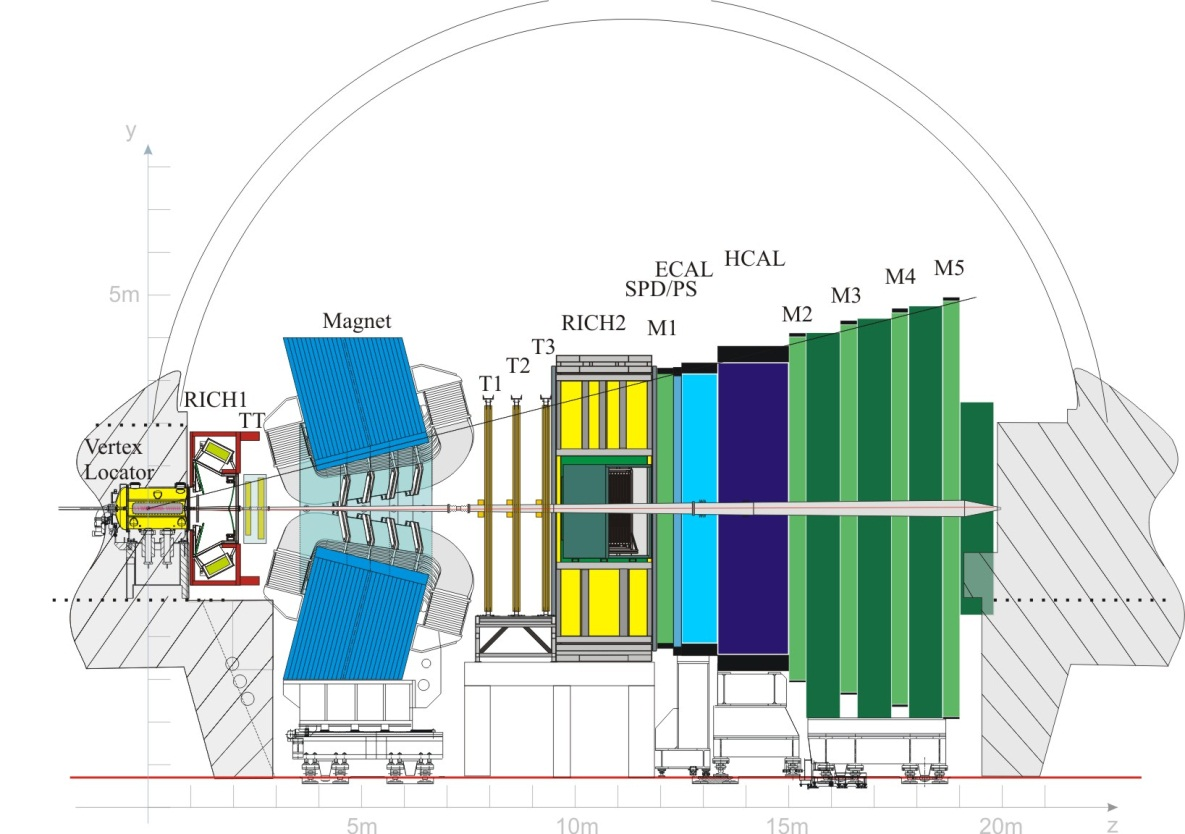
\includegraphics[width=80mm]{5x0vbq.jpg}
	\caption{The structure of the LHCb detector \label{aaa}}
\end{figure}

The detector is $21$ metres long, $10$ metres high and $13$ metres wide, and sits $100$ metres below ground near the town of Ferney-Voltaire, France.

\subsection{Physics goals of the exercise}

The data sample used for this exercise consists of candidates for a type of charmed particle known as a $D^0$ meson found in a sample of randomly collected LHC interactions during 2011 data-taking. A $D^0$ particle consists of a charm quark and an up antiquark. The particles are measured decaying in the mode:
$$D^{0}\rightarrow K^{-}\pi ^{+}$$
where the final state particles are a kaon $K^{-}$ consisting of a strange quark and an up antiquark, and a pion which consists of a down antiquark and an up quark (fig.~\ref{d1}).
\begin{figure}[ht!]
	\centering
	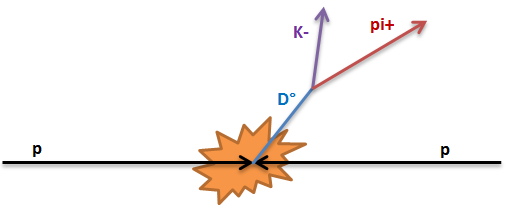
\includegraphics[width=80mm]{25grrk4.png}
	\caption{The $D^0$ decay directly from the proton - proton collision \label{d1}}
\end{figure}
The objects of this exercise, $D^0$ particles, have a distinctive feature and that is their measurably long lifetime. The average lifetime of a $D^0$ meson is $4\cdot 10^{-13}$ seconds. It travels nearly at the speed of light at LHCb, typically: $v\approx 0.99919\cdot c$. Therefore the average distance travelled is expected to be:
$$0.4 ~\beta ~\gamma ~c =3 ~\mathrm{mm}.$$
where $~\gamma$ is the Lorentz factor. Fast mesons live longer, thus a lifetime at rest of $0.4$ ~ps means a lifetime inside the experiment of about $10$ ~ps or even longer. The $D^0$ particle can also appear as a child of a $B$ particle. In that case we measure the displacement as the impact parameter (IP) which is the perpendicular distance between the path of the $D^0$ particle and the center of the collision. When the $D^0$ particle comes from the primary vertex the IP is small, but when it comes from the secondary vertex it is large, as shown in the figure ~\ref{d2}. This fact, together with their abundant production, allows the $D^0$ signals to be well separated from the background of the underlying event, most of which consists of random combinations of particles produced in the proton-proton collision.

\begin{figure}[ht!]
	\centering
	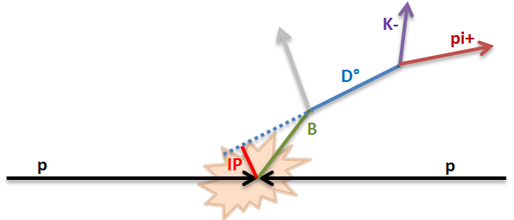
\includegraphics[width=80mm]{311up94pro.jpg}
	\caption{Secondary verteces that are displaced from the proton - proton collision \label{d2}}
\end{figure}

\subsection{The invariant mass calculation}
The invariant mass (``rest mass'') is defined as an invariant quantity which is the same for all observers in all reference frames. It can be calculated using the Energy $E$ and Momentum $p$ measured in the detector. Here is the derivation of the formula for the invariant mass: \par
Conservation of energy: $$E=E_{1}+E_{2}$$
Conservation of momentum: $$\overrightarrow{p}=\overrightarrow{p_{1}}+\overrightarrow{p_{2}}$$
From relativity (where we set c=1): $$\left ( pc \right )^{2}+\left ( mc^{2} \right )^{2}=E^{2}$$
$$E^{2}=p^{2}+m^{2}$$
From the previous equations: $$m^{2}=E^{2}-p^{2}=\left ( E_{1}+E_{2} \right )^{2}-\left \| p_{1}+p_{2} \right \|$$ 
$$=\left ( E_{1}+E_{2} \right )^{2}-\left (\overrightarrow{p_{1}}+\overrightarrow{p_{2}}  \right )\cdot \left ( \overrightarrow{p_{1}}+\overrightarrow{p_{2}} \right )$$
The dot product of two orthogonal vectors is zero. Therefore the invariant mass is:
$$m^{2}=\left ( E_{1}+E_{2} \right )^{2}-\left ( p_{1x}+p_{2x} \right )^{2}-\left ( p_{1y}+p_{2y} \right )^{2}-\left ( p_{1z}+p_{2z} \right )^{2}$$
The goal for the students is to calculate the invariant mass of two chosen particles and if the mass is close to the $D^{0}$ mass, add it to a histogram.
\section{Implementation}
\subsection{Timeline}
The LHCb Event Display was fully developed, tested and integrated with existing application during the time period from July 2013 to December 2013. It was actively used by students who participated in the International Masterclass program in March 2014.
\begin{figure}[ht!]
	\centering
	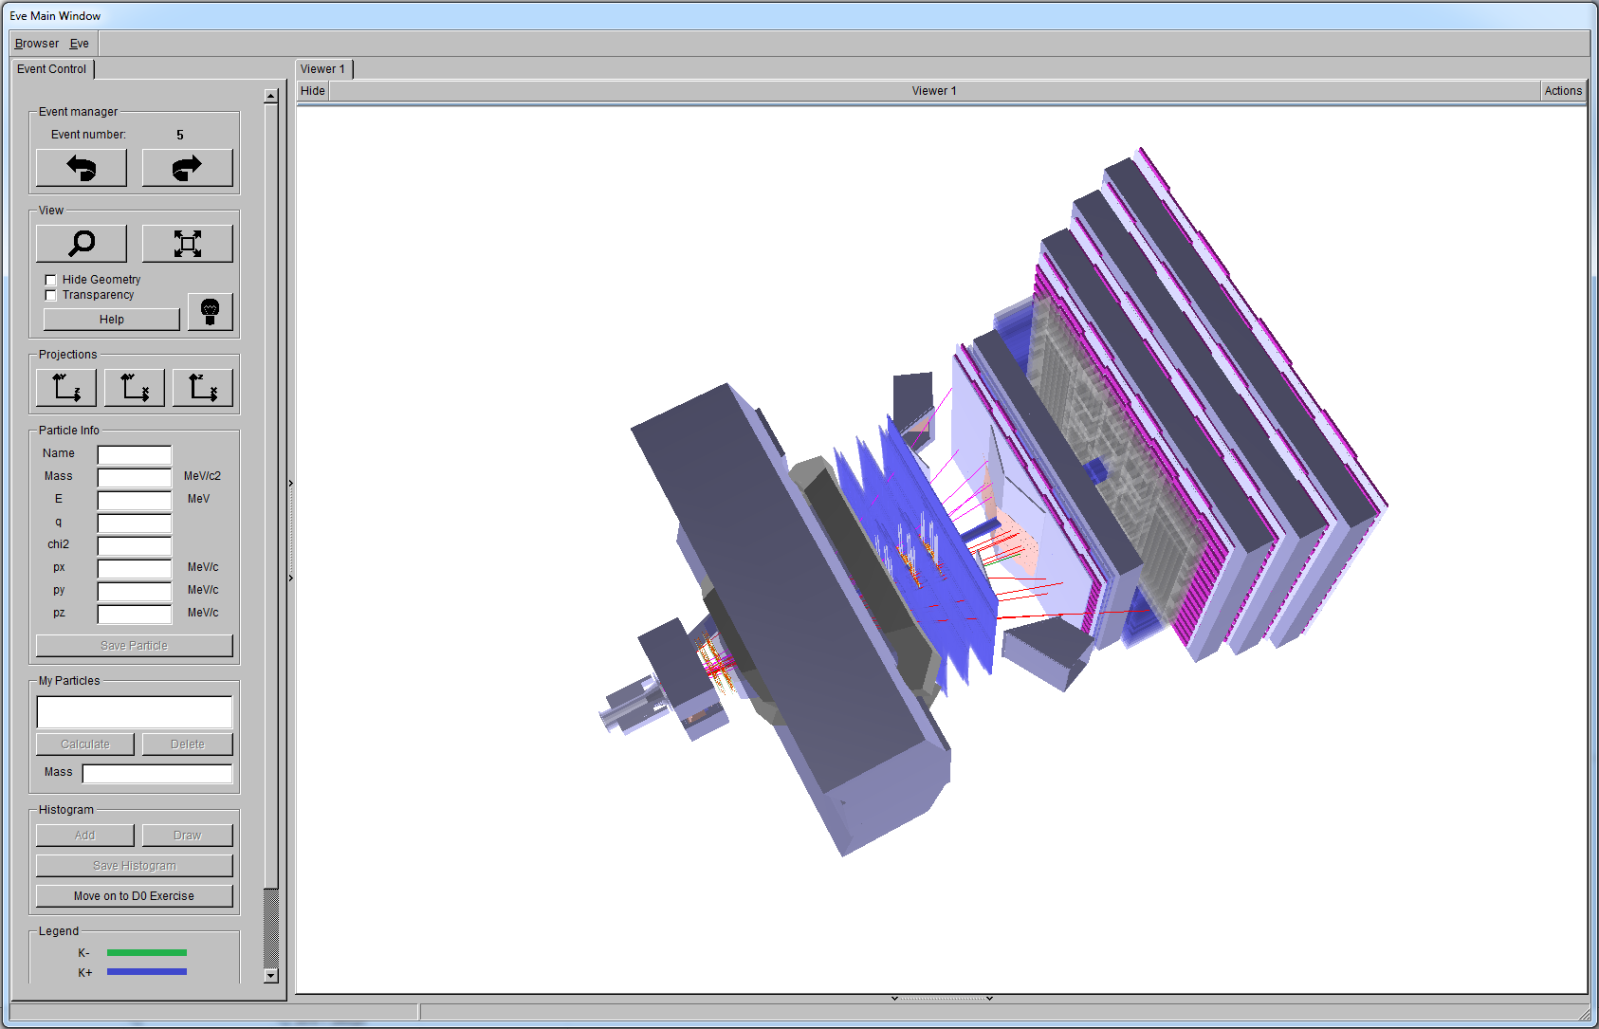
\includegraphics[width=80mm]{2rr2gid.png}
	\caption{The full appearance of the LHCb Event Display for the Masterclass exercise \label{o5}}
\end{figure}
\subsection{ROOT framework}
ROOT is an object-oriented data analysis framework, written in C++. It contains several tools designed for statistical data exploration, fitting and reporting. Significantly for this project, ROOT comes with powerful graphics capabilities and interfaces, including an extensive and self-contained graphical user interface (GUI) development kit that can be used to develop easy-to-use customized interfaces for the end users. ROOT was developed at CERN as it was needed to address the challenge posed by the experimental high energy physics community, where scientists produce and analyse vast amounts of very complex data. \par
ROOT provides GUI tools for developing user interfaces based on the ROOT GUI classes. It includes over 30 widgets (i.e. text box, button, check box etc.) and aims to offer a complete set of features needed for developing the GUI projects. The GUI builder offers a palette of user interface elements. They can be selected, positioned, grouped and laid out in the main application frame. The main menu and palette for the application were created using the ROOT GUI builder. The icons which were used were custom-made for this purpose.\par
ROOT was used as a developing tool for this application because the base of the Masterclass exercise was done in ROOT and because the geometry of LHCb detector, which was needed for the Display, was already available in ROOT. Additionally, ROOT is an open-source framework therefore it does not require any licence or special permissions. 

\section{Motivation}
\subsection{Goals}
This exercise was designed to teach the students how to use an event display of the proton-proton collision inside the LHCb detector to search for charmed particles.
Students should:
\begin{itemize}
\setlength{\itemsep}{0pt}
	\item Learn to use an event display to identify displaced vertices.
	\item Understand the problem of statistics in the LHCb experiment. A large number of events are needed to see the signal and reduce the statistical uncertainty.
	\item Learn to use histograms and fits.
	\item Understand signal significance.
	\item Learn about systematic uncertainties in measurements. 
\end{itemize}
\subsection{Guide through the exercise}
The aim of the event display exercise is to locate displaced vertices belonging to $D^0$ particles in the vertex detector of the LHCb experiment. When the exercise is launched and an event is loaded, an image of the LHCb detector appears with particle trajectories inside it (fig.~\ref{o5}). These tracks are colour-coded, and a legend at the bottom of the GUI shows which colour corresponds to which kind of particle.

In order to make identifying vertices easier, the GUI allows the viewing of an event in three different two-dimensional projections: $y-z$, $y-x$, and $x-z$. Displaced vertices appear as a pair of intersecting tracks, far away from the other tracks in the event. When a particle is selected, its information, including mass and momentum, will appear in the Particle Info box.\par
A $D^0$ particle decays into a kaon and a pion, so students will need to find a displaced vertex where a kaon track intersects with a pion track. Once they find a track which they think is part of the displaced vertex, they can save its information. When the students have collected two particles, they can compute the invariant mass and if this combination has a mass compatible with mass of the $D^0$ particle, then it will be added on a histogram. By saving a combination for each event, the student will build up the histogram of the masses of the displaced vertices in the different events (fig.~\ref{o8}).\par
\begin{figure}[ht!]
	\centering
	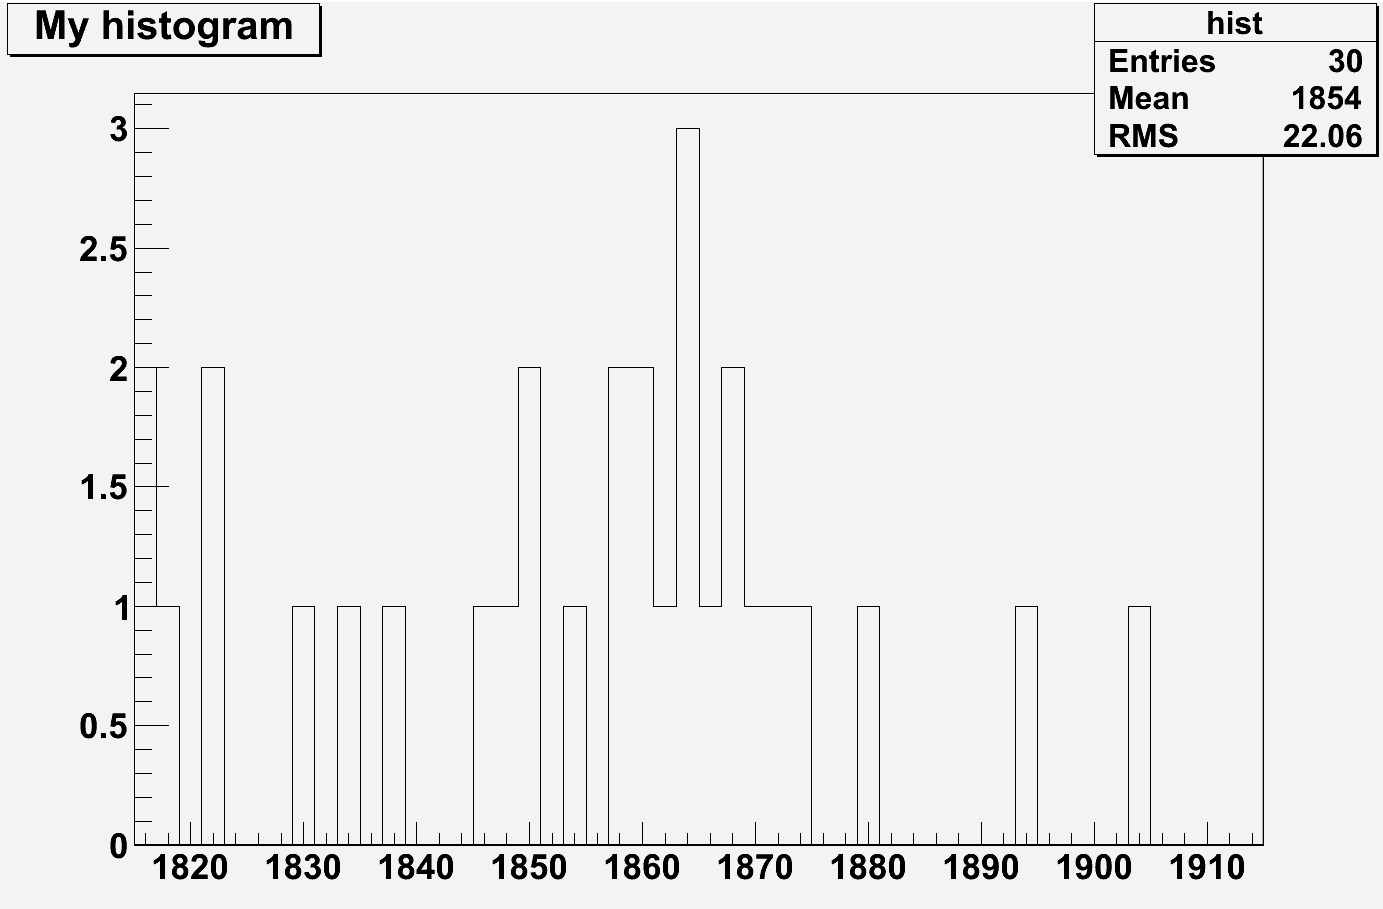
\includegraphics[width=70mm]{2198k7c.png}
	\caption{Built-up histogram of the invariant masses. Final result of the exercise obtained by a student. \label{o8}}
\end{figure}
Since the data is real, it contains both signal and background. The detector has a finite resolution, so not all displaced vertices will have exactly the $D^0$ mass (even the signal ones). They should, however, be within the range $1816-1914 ~MeV$ (this range is around $3\%$ each way around the known $D^0$ mass). If students try to save a combination which is too far away from the real $D^0$ mass (which means that they have not found the correct displaced vertex pair) the exercise will warn them that about it and will not add the mass to the histogram.

Students can switch through events, so if they are not able to find the displaced vertex for an event after a few minutes, they can come back to it at the end of the exercise. Once they have looked at all events, they can examine the fully built mass histogram. The shape in the histogram should be discussed with a teacher or a moderator. At the end, students should save the histogram to disk. It will then be combined by the moderators with the histograms of the other students, all together, students and moderators should discuss the results as a group.

The following flow chart (fig.~\ref{o9}) represents the exercise workflow:
\begin{figure}[ht!]
	\centering
	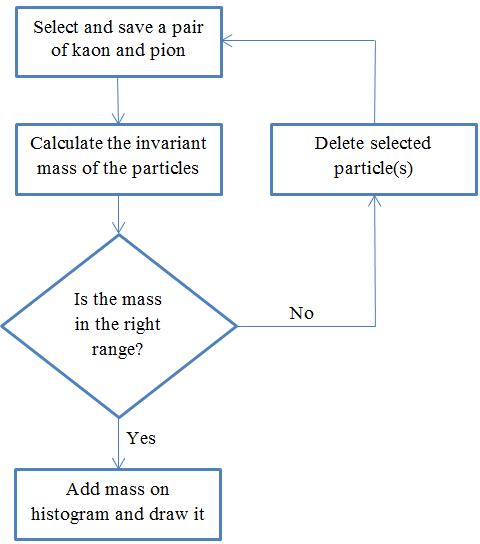
\includegraphics[width=70mm]{29o1h1w.png}
	\caption{Algorithm for analysing a single event \label{o9}}
\end{figure}

%% The Appendices part is started with the command \appendix;
%% appendix sections are then done as normal sections
%% \appendix

%% \section{}
%% \label{}

\section{Architecture}
The core of the application is the class \textit{Frame} and the class \textit{ParticleTrack}. Both of them use many other built-in classes to achieve the functionality required by the exercise. The objective of class \textit{Frame} is divided into a number of separate and independent segments which contribute to the final purpose of the application. These segments are:
\begin{itemize}
\setlength{\itemsep}{0pt}
	\item Initial settings
	\item Geometry manager
	\item Event manager
	\item Navigation manager
	\item Histogram manager 
\end{itemize}
The class \textit{ParticleTrack} contains all the information about a particle and its path. An array of these instances in the code presents a set of particles originated from the same collision and that is an event in the Event Display. 
\subsection{Initial settings}
Methods from the initial settings segment are called when the application is launched. They set the environment and create the GUI. For example: height and width of the main window are set to be 90\% of the screen size during the initialization.\par

\subsection{Geometry manager}
The geometry manager controls the camera and elements on the screen of the Event Display. In the beginning, the camera is set to be in the starting position where the full look of LHCb detector is displayed. Using the options from the menu students can hide the geometry or see it transparently. In addition, when students want to observe the collision point, this manager can set the camera near the collision point in orthographic projections --- $YZ$, $YX$ and $YX$.\par
Every element on the display is shown through the Event Visualization Environment of ROOT, also known as EVE, an application framework for construction of event-display programs. It is built on top of ROOT's GUI, OpenGL, and GED (the ROOT Graphics Editor) infrastructure. It offers the base-classes for representation of visual objects that can be presented in list-tree views, object-editors and rendered via OpenGL. Furthermore it has an application manager class TEveManager for top-level management of elements, GUI components, geometries and events. \par
In order to link every particle track from the screen with its own particle information we used a data structure called map. Maps are associative containers that store elements formed by a combination of a key value and a mapped value, following a specific order. In this case the key value is a float, usually named index, and the mapped value is an instance of the class \textit{ParticleTrack} that contains all needed information about a particle. In a map, the key values are generally used to sort and uniquely identify the elements, while the mapped values store the content associated to this key.

\subsection{Event manager}
The event manager handles events in the Display. There are thirty events for every student to analyze. Students can go back and forth through the events using the buttons on the screen. On the button click, the event manager will first clear the screen of the previous event and then load the next set of particles. Finally, it will clear the Particle Info Box and regulate availability of the buttons. Particle Info Box is a part of the GUI which displays information about a selected particle.
\subsection{Navigation manager}
The navigation manager guides the students through the exercise by gradually increasing their privileges on the form. In the beginning most of the buttons are disabled. As students select particles and save them, other buttons become enabled, and students can press on them in order to complete the exercise. 
\subsection{Histogram manager}
When a student wants to examine the histogram of the invariant masses, this manager opens a new tab in the application and draws the histogram in it. If the tab is already open, the histogram will be just updated. \par
Furthermore, this histogram can be saved on the hard disk drive, because ROOT offers the possibility to write the instances of all the classes in ROOT on disk, into what is referred to as a ROOT file. One says that the object is made ``persistent'' by storing it on disk. When reading the file back, the object will be restored to memory.

\section{Conclusion}
This project was a significant success due to the fact that the LHCb experiment was admitted to the International Masterclass programme for the first time.\par
During the time period from 12\textsuperscript{th} March to 3\textsuperscript{rd} April, more than twenty institutes participated in the LHCb Masterclass Exercise with more than 500 students all together. Institutes were from the United Kingdom, the United States, France, Italy, Romania, Germany and the Netherlands. The exercise was translated into all of the national languages, except Dutch, because tutors from the Netherlands stated that their students were very familiar with English.\par
Students who have used a final version of the applications stated that they found it interactive and satisfying. We have received a lot of positive feedback from the participating institutes and the students. These feedback prove that our solution met the standard and the requirements of the International Masterclass programme. 

\section{Further work}
An official upgrade of the current event display is called the Total Event Visualizer (TEV) (fig.~\ref{o2}). It is supposed to have event displays for all the experiments at the LHC integrated in one application. As seen on the figure ~\ref{o1}, every experiment should be handled in the same way: with the same operation classes and the common event structure. The major challenge lies in implementing the data translator which should be able to handle data from every experiment. From the shared GUI, a user should be able to choose the experiment and get the information and the data from it.\par
\begin{figure}[ht!]
	\centering
	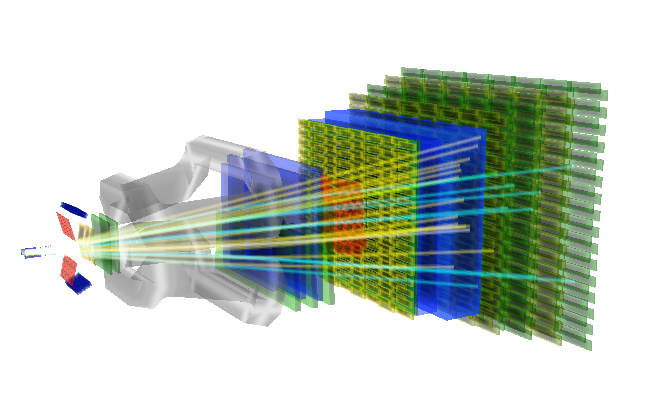
\includegraphics[width=80mm]{2r6l6zd.png}
	\caption{Full appearance of the LHCb detector in TEV \label{o2}}
\end{figure}
TEV is based on computing gaming technology and is implemented in Unity Pro (version 4.3.4). The major advantage is suitability with many platforms including Windows, Mac OS, iOS, Android and also a web player. Regarding to the appearance, the main objectives of TEV are: 
\begin{enumerate}
	  \item It should be easy to use
	  \item It should be visually appealing
	  \item It should engage users the right way
	  \item It should be flexible and usable in many scenarios
\end{enumerate}
\begin{figure}[ht!]
	\centering
	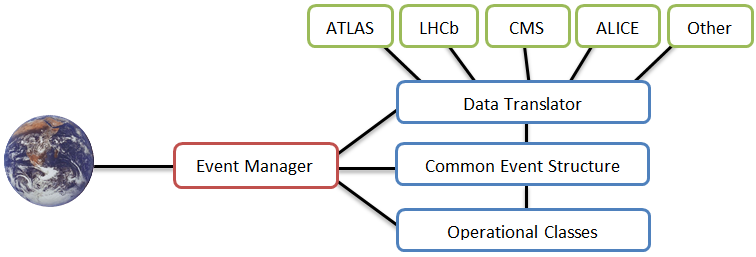
\includegraphics[width=80mm]{2u4r5es.png}
	\caption{The structure of the Total Event Visualizer (TEV)\label{o1}}
\end{figure}
The new application should have many purposes: it will be used as a scientific discovery tool for general public, as an International Masterclass exercise for high-school students, and even for minor professional purposes. One of the plans for future work would be integrating facility from ROOT into TEV.

\section*{Acknowledgements}
I would like to express my very great appreciation to my supervisor, Vladimir Gligorov, for the valuable guidance and advice. I would like to offer my special thanks to Ben Couturier and Thomas Blake to for their contribution to this project.  Also, I would like to thank Despina Hatzifotiadou for supporting us during the early stages of the project and Sava Cajetinac (Microsoft Development Centre Serbia) for the useful aesthetic tips and design of the ``Help'' pages.

%% References
%%
%% Following citation commands can be used in the body text:
%% Usage of \cite is as follows:
%%   \cite{key}         ==>>  [#]
%%   \cite[chap. 2]{key} ==>> [#, chap. 2]
%%

%% References with BibTeX database:
\nocite{*}
\bibliographystyle{elsarticle-num}
%\bibliography{martin}
\begin{thebibliography}{8}
	\bibitem{officialguide} LHCb Masterclass: \emph{Measuring the $D^0$ lifetime at the LHC, official guide through the exercise}, (2013).Available at: \url{http://lhcb-public.web.cern.ch/lhcb-public/en/LHCb-outreach/masterclasses/ENinstructions.pdf} (Accessed: May 2014).
	\bibitem{cpp} C++ documentation (2000-2014.) Available at: \url{http://www.cplusplus.com/reference/map/map/} (Accessed: 5 May 2014).
	\bibitem{root} ROOT: \emph{A Data Analysis and Data Mining Tool from CERN, an introductory guide for ROOT}. Available at: \url{https://www.casact.org/pubs/forum/08wforum/kumar_tripathi.pdf} (Accessed: 8 May 2014).
	\bibitem{alice} Looking for strange particles in ALICE, official website for ALICE Masterclass exercise. Available at: \url{http://aliceinfo.cern.ch/public/MasterCL/webpage-masterclass.html}  (Accessed: 8 May 2014).
	\bibitem{lhcb} Official website of LHCb experiment at CERN. Available at: \url{http://home.web.cern.ch/about/experiments/lhcb} (Accessed: 12 May 2014).
	\bibitem{lhcbwebsite} HEP: \emph{An Educational Tour in the LHCb Experiment}. Available at: \url{http://hepoutreach.syr.edu/HEP_Tour/lhcbexperiment/index.html} (Accessed: 12 May 2014).
	\bibitem{rootVisStud} ROOT and Visual Studio. Available at: \url{https://twiki.cern.ch/twiki/bin/view/Sandbox/ROOTandVisualStudio#_Toc336335692} (Accessed: 14 May 2014).
	\bibitem{eve} EVE --- Event Visualization Environment of the ROOT framework. Available at: \url{http://pos.sissa.it//archive/conferences/070/103/ACAT08_103.pdf} (Accessed: 20 May 2014).
\end{thebibliography}

%% Authors are advised to use a BibTeX database file for their reference list.
%% The provided style file elsarticle-num.bst formats references in the required Procedia style

%% For references without a BibTeX database:

% \begin{thebibliography}{00}

%% \bibitem must have the following form:
%%   \bibitem{key}...
%%

% \bibitem{}

% \end{thebibliography}

\end{document}

%%
%% End of file `nuphbp-template.tex'. 
